\documentclass[english, 11 pt, class=article, crop=false]{standalone}
%%


\newcommand{\note}{Merk}

\usepackage[T1]{fontenc}
%\renewcommand*\familydefault{\sfdefault} % For dyslexia-friendly text
\usepackage{lmodern} % load a font with all the characters
\usepackage{geometry}
\geometry{verbose,paperwidth=16.1 cm, paperheight=24 cm, inner=2.3cm, outer=1.8 cm, bmargin=2cm, tmargin=1.8cm}
\setlength{\parindent}{0bp}
\usepackage{import}
\usepackage[subpreambles=false]{standalone}
\usepackage{amsmath}
\usepackage{amssymb}
\usepackage{esint}
\usepackage{babel}
\usepackage{tabu}
\makeatother
\makeatletter

\usepackage{titlesec}
\usepackage{ragged2e}
\RaggedRight
\raggedbottom
\frenchspacing

% Norwegian names of figures, chapters, parts and content
\addto\captionsenglish{\renewcommand{\figurename}{Figur}}
\makeatletter
\addto\captionsenglish{\renewcommand{\chaptername}{Kapittel}}
\addto\captionsenglish{\renewcommand{\partname}{Del}}


\usepackage{graphicx}
\usepackage{float}
\usepackage{subfig}
\usepackage{placeins}
\usepackage{cancel}
\usepackage{framed}
\usepackage{wrapfig}
\usepackage[subfigure]{tocloft}
\usepackage[font=footnotesize,labelfont=sl]{caption} % Figure caption
\usepackage{bm}
\usepackage[dvipsnames, table]{xcolor}
\definecolor{shadecolor}{rgb}{0.105469, 0.613281, 1}
\colorlet{shadecolor}{Emerald!15} 
\usepackage{icomma}
\makeatother
\usepackage[many]{tcolorbox}
\usepackage{multicol}
\usepackage{stackengine}

\usepackage{esvect} %For vectors with capital letters

% For tabular
\usepackage{array}
\usepackage{multirow}
\usepackage{longtable} %breakable table

% Ligningsreferanser
\usepackage{mathtools}
\mathtoolsset{showonlyrefs}

% index
\usepackage{imakeidx}
\makeindex[title=Indeks]

%Footnote:
\usepackage[bottom, hang, flushmargin]{footmisc}
\usepackage{perpage} 
\MakePerPage{footnote}
\addtolength{\footnotesep}{2mm}
\renewcommand{\thefootnote}{\arabic{footnote}}
\renewcommand\footnoterule{\rule{\linewidth}{0.4pt}}
\renewcommand{\thempfootnote}{\arabic{mpfootnote}}

%colors
\definecolor{c1}{cmyk}{0,0.5,1,0}
\definecolor{c2}{cmyk}{1,0.25,1,0}
\definecolor{n3}{cmyk}{1,0.,1,0}
\definecolor{neg}{cmyk}{1,0.,0.,0}

% Lister med bokstavar
\usepackage[inline]{enumitem}

\newcounter{rg}
\numberwithin{rg}{chapter}
\newcommand{\reg}[2][]{\begin{tcolorbox}[boxrule=0.3 mm,arc=0mm,colback=blue!3] {\refstepcounter{rg}\phantomsection \large \textbf{\therg \;#1} \vspace{5 pt}}\newline #2  \end{tcolorbox}\vspace{-5pt}}

\newcommand\alg[1]{\begin{align} #1 \end{align}}

\newcommand\eks[2][]{\begin{tcolorbox}[boxrule=0.3 mm,arc=0mm,enhanced jigsaw,breakable,colback=green!3] {\large \textbf{Eksempel #1} \vspace{5 pt}\\} #2 \end{tcolorbox}\vspace{-5pt} }

\newcommand{\st}[1]{\begin{tcolorbox}[boxrule=0.0 mm,arc=0mm,enhanced jigsaw,breakable,colback=yellow!12]{ #1} \end{tcolorbox}}

\newcommand{\spr}[1]{\begin{tcolorbox}[boxrule=0.3 mm,arc=0mm,enhanced jigsaw,breakable,colback=yellow!7] {\large \textbf{Språkboksen} \vspace{5 pt}\\} #1 \end{tcolorbox}\vspace{-5pt} }

\newcommand{\sym}[1]{\colorbox{blue!15}{#1}}

\newcommand{\info}[2]{\begin{tcolorbox}[boxrule=0.3 mm,arc=0mm,enhanced jigsaw,breakable,colback=cyan!6] {\large \textbf{#1} \vspace{5 pt}\\} #2 \end{tcolorbox}\vspace{-5pt} }

\newcommand\algv[1]{\vspace{-11 pt}\begin{align*} #1 \end{align*}}

\newcommand{\regv}{\vspace{5pt}}
\newcommand{\mer}{\textsl{Merk}: }
\newcommand{\mers}[1]{{\footnotesize \mer #1}}
\newcommand\vsk{\vspace{11pt}}
\newcommand\vs{\vspace{-11pt}}
\newcommand\vsb{\vspace{-16pt}}
\newcommand\sv{\vsk \textbf{Svar} \vspace{4 pt}\\}
\newcommand\br{\\[5 pt]}
\newcommand{\figp}[1]{../fig/#1}
\newcommand\algvv[1]{\vs\vs\begin{align*} #1 \end{align*}}
\newcommand{\y}[1]{$ {#1} $}
\newcommand{\os}{\\[5 pt]}
\newcommand{\prbxl}[2]{
\parbox[l][][l]{#1\linewidth}{#2
	}}
\newcommand{\prbxr}[2]{\parbox[r][][l]{#1\linewidth}{
		\setlength{\abovedisplayskip}{5pt}
		\setlength{\belowdisplayskip}{5pt}	
		\setlength{\abovedisplayshortskip}{0pt}
		\setlength{\belowdisplayshortskip}{0pt} 
		\begin{shaded}
			\footnotesize	#2 \end{shaded}}}

\renewcommand{\cfttoctitlefont}{\Large\bfseries}
\setlength{\cftaftertoctitleskip}{0 pt}
\setlength{\cftbeforetoctitleskip}{0 pt}

\newcommand{\bs}{\\[3pt]}
\newcommand{\vn}{\\[6pt]}
\newcommand{\fig}[1]{\begin{figure}
		\centering
		\includegraphics[]{\figp{#1}}
\end{figure}}

\newcommand{\figc}[2]{\begin{figure}
		\centering
		\includegraphics[]{\figp{#1}}
		\caption{#2}
\end{figure}}

\newcommand{\sectionbreak}{\clearpage} % New page on each section

\newcommand{\nn}[1]{
\begin{equation}
	#1
\end{equation}
}

% Equation comments
\newcommand{\cm}[1]{\llap{\color{blue} #1}}

\newcommand\fork[2]{\begin{tcolorbox}[boxrule=0.3 mm,arc=0mm,enhanced jigsaw,breakable,colback=yellow!7] {\large \textbf{#1 (forklaring)} \vspace{5 pt}\\} #2 \end{tcolorbox}\vspace{-5pt} }
 
%colors
\newcommand{\colr}[1]{{\color{red} #1}}
\newcommand{\colb}[1]{{\color{blue} #1}}
\newcommand{\colo}[1]{{\color{orange} #1}}
\newcommand{\colc}[1]{{\color{cyan} #1}}
\definecolor{projectgreen}{cmyk}{100,0,100,0}
\newcommand{\colg}[1]{{\color{projectgreen} #1}}

% Methods
\newcommand{\metode}[2]{
	\textsl{#1} \\[-8pt]
	\rule{#2}{0.75pt}
}

%Opg
\newcommand{\abc}[1]{
	\begin{enumerate}[label=\alph*),leftmargin=18pt]
		#1
	\end{enumerate}
}
\newcommand{\abcs}[2]{
	\begin{enumerate}[label=\alph*),start=#1,leftmargin=18pt]
		#2
	\end{enumerate}
}
\newcommand{\abcn}[1]{
	\begin{enumerate}[label=\arabic*),leftmargin=18pt]
		#1
	\end{enumerate}
}
\newcommand{\abch}[1]{
	\hspace{-2pt}	\begin{enumerate*}[label=\alph*), itemjoin=\hspace{1cm}]
		#1
	\end{enumerate*}
}
\newcommand{\abchs}[2]{
	\hspace{-2pt}	\begin{enumerate*}[label=\alph*), itemjoin=\hspace{1cm}, start=#1]
		#2
	\end{enumerate*}
}

% Oppgaver
\newcommand{\opgt}{\phantomsection \addcontentsline{toc}{section}{Oppgaver} \section*{Oppgaver for kapittel \thechapter}\vs \setcounter{section}{1}}
\newcounter{opg}
\numberwithin{opg}{section}
\newcommand{\op}[1]{\vspace{15pt} \refstepcounter{opg}\large \textbf{\color{blue}\theopg} \vspace{2 pt} \label{#1} \\}
\newcommand{\ekspop}[1]{\vsk\textbf{Gruble \thechapter.#1}\vspace{2 pt} \\}
\newcommand{\nes}{\stepcounter{section}
	\setcounter{opg}{0}}
\newcommand{\opr}[1]{\vspace{3pt}\textbf{\ref{#1}}}
\newcommand{\oeks}[1]{\begin{tcolorbox}[boxrule=0.3 mm,arc=0mm,colback=white]
		\textit{Eksempel: } #1	  
\end{tcolorbox}}
\newcommand\opgeks[2][]{\begin{tcolorbox}[boxrule=0.1 mm,arc=0mm,enhanced jigsaw,breakable,colback=white] {\footnotesize \textbf{Eksempel #1} \\} \footnotesize #2 \end{tcolorbox}\vspace{-5pt} }
\newcommand{\rknut}{
Rekn ut.
}

%License
\newcommand{\lic}{\textit{Matematikken sine byggesteinar by Sindre Sogge Heggen is licensed under CC BY-NC-SA 4.0. To view a copy of this license, visit\\ 
		\net{http://creativecommons.org/licenses/by-nc-sa/4.0/}{http://creativecommons.org/licenses/by-nc-sa/4.0/}}}

%referances
\newcommand{\net}[2]{{\color{blue}\href{#1}{#2}}}
\newcommand{\hrs}[2]{\hyperref[#1]{\color{blue}\textsl{#2 \ref*{#1}}}}
\newcommand{\rref}[1]{\hrs{#1}{regel}}
\newcommand{\refkap}[1]{\hrs{#1}{kapittel}}
\newcommand{\refsec}[1]{\hrs{#1}{seksjon}}

\newcommand{\mb}{\net{https://sindrsh.github.io/FirstPrinciplesOfMath/}{MB}}


%line to seperate examples
\newcommand{\linje}{\rule{\linewidth}{1pt} }

\usepackage{datetime2}
%%\usepackage{sansmathfonts} for dyslexia-friendly math
\usepackage[]{hyperref}


\begin{document}
	
	
	
\section{Knapper og kommandoer}
\subsection*{Grafikkfelt}
Knappene velges fra rullemenyer på verktøylinjen. Nummereringen av menyene er fra venstre.\vsk

\begin{tabular}{@{}l}
	\,
\includegraphics[scale=0.4]{fig/pkt} Lager et nytt punkt. (Meny nr. 1) \\
	\,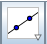
\includegraphics[scale=0.4]{fig/lin} Lager linje mellom to punkt. (Meny nr. 2)\\	
	\,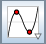
\includegraphics[scale=0.4]{fig/ekst} Finner topp- og bunnpunkt til en funksjon. (Meny nr. 2)\\
	\,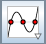
\includegraphics[scale=0.4]{fig/nul} Finner nullpunktene til en funksjon. (Meny nr. 2)	\\
	\,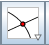
\includegraphics[scale=0.4]{fig/skj} Finner skjæringspunkt mellom to objekt. (Meny nr. 3)\\	
	\,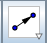
\includegraphics[scale=0.4]{fig/vek} Lager vektoren mellom to punkt (Meny nr. 3)\\		
	\,
\includegraphics[scale=0.4]{fig/tekst} Lager en tekstboks. (Meny nr. 10)\\		
	\,
\includegraphics[scale=0.4]{fig/flytt} Flytter grafikkfeltet. Endrer verdiavstanden hvis man peker på aksene. \\
	\hspace{1cm}(Meny nr. 10)\\			
\end{tabular}
\subsubsection*{CAS}
\begin{tabular}{@{}l}
	\;
\includegraphics[scale=0.4]{fig/erlik} Gjengir uttrykket som er inntastet, ofte i forkortet form.\\	
	\;
\includegraphics[scale=0.4]{fig/brin} Gjengir uttrykket som er inntastet.\\	
	\;
\includegraphics[scale=0.4]{fig/caerlik} Gir tilnærmet verdi av et uttrykk (som desimaltall). \\	
	\;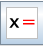
\includegraphics[scale=0.4]{fig/x} Gir eksaktløsningen av en ligning.\\
	\;
\includegraphics[scale=0.4]{fig/xca} Gir tilnærmet løsning av en ligning som desimaltall.\\
	
\end{tabular}

\subsubsection{Hurtigtaster}
\begin{tabular}{@{}c | c |c | c }
	&\textbf{Beskrivelse} & \textbf{PC }& \textbf{Mac} \\ \hline
	$ \sqrt{} $	& kvadratrot& \texttt{alt\,+\,r} &\texttt{alt\,+\,r} \\\hline
	$ \pi $	& pi& \texttt{alt\,+\,p} & \texttt{alt\,+\,p}\\\hline
	$ \infty $ &uendelig& \texttt{alt\,+\,u} &\texttt{alt\,+\,,}  \\\hline
	$ \otimes $&kryssprodukt & \texttt{alt\,+\,shift\,+\,8}&\texttt{ctrl\,+\,shift\,+\,8} \\\hline
	$ e $&eulers tall & \texttt{alt\,+\,e}& \texttt{alt\,+\,e}\\\hline
	$ {}^\circ $&gradtegnet ($ \frac{\pi}{180} $) & \texttt{alt\,+\,o}& \texttt{alt\,+\,o}
	\\\hline	
\end{tabular}
\newpage
\subsubsection{Kommandoliste}
\cm{abs}{<x>}
{Finner lengden til et objekt \textit{x}.
}

\cm{Asymptote}{<Funksjon>}
{Finner asymptotene til en funksjon.}

\cm{Avstand}{<Punkt>, <Objekt>}
{Gir avstanden fra et punkt til et objekt.}

\cmc{ByttUt}{<Uttrykk>, <Liste med forandringer>}
{Viser et gitt uttrykk etter endring av variabler, gitt i en liste.}

\cm{Deriverte}{<Funksjon>}	
{Gir den deriverte av en funksjon.
	
	\mers{
		For en definert funksjon $ f(x) $, kan man like gjerne skrive \texttt{f'(x)}.
}}

\cm{Ekstremalpunkt}{<Funksjon>, <Start>, <Slutt> } {Finner lokale ekstremalpunkt og ekstremalverdier for en funksjon $ f $ på et gitt intervall.}

\cm{Ekstremalpunkt}{Polynom}
{Finner lokale ekstremalpunkt og ekstremalverdier til et polynom.}

\cm{Funksjon}{<Funksjon>, <Start>, <Slutt>}
{Tegner en funksjon på et gitt intervall.}

\cm{Høyde}{<Objekt>}
{Gir avstanden fra toppunkt til grunnflate i et objekt. 
	\mers{Avstanden har retning, og derfor kan den noen ganger være negativ. Tallverdien er den geometriske høyden.}}

\cmc{HøyreSide}{<Likning>}
{Gir høyresiden til en likning.}

\cmc{HøyreSide}{<Liste med likninger>}
{Gir en liste med høyresidene i en liste med ligninger.}

\cm{Integral}{<Funksjon>}
{Gir uttrykket til det ubestemte integralet av en funksjon. (Merk: Hvis kommandoen skrives i inntastingsfeltet, blir konstantleddet utelatt).}

\cm{Integral}{<Funksjon>, <Start>, <Slutt>}
{Gir det bestemte integralet av en funksjon på et intervall.}

\cmc{Integral}{<Variabel>}
{Gir uttrykket til det ubestemte integralet til en funksjon av gitt variabel. (Brukes dersom man ønsker å integrere funksjoner avhengig av en annen variabel enn $ x $).}

\cm{Kule}{<Punkt>, <Radius>}
{Viser en kule i Grafikkfelt 3D med sentrum i et gitt punkt og med en gitt radius.}

\cm{Kurve}{<Uttrykk>, <Uttrykk>, <Uttrykk>, <Parametervariabel>, <Start>, <Slutt>}
{Viser parameteriseringen av en kurve i Grafikkfelt 3D på et gitt intervall. Uttrykkene er henholdsvis uttrykkene for $ {x, y} $ og $ z $-koordinatene, bestemt av en gitt parametervariabel.
	
\mers{
Med mindre et bestemt intervall av kurven er ønsket, er det bedre å skrive parameteriseringen direkte inn i inntastingsfeltet som \texttt{A+t*u}, hvor $ A $ er et punkt på linja og $ u$ er en retningsvektor.
}}

\cm{Linje}{<Punkt>, <Punkt>}{ Gir uttrykket til en linje mellom to punkt. Hvis punktene har tre koordinater besår uttrykket av et punkt på linja og en fri variabel $ \}lambda $ mulitplisert med en retningsvektor.}

\cmc{Løs}{<Likning med x>}{
Løser en likning med $ x $ som ukjent.
}

\cmc{Løs}{<Liste med likninger>, <Liste med variabler>}
{Finner alle løsninger av en liste med ligninger med gitte variabel som ukjente.}

\cmc{Løs}{<Likning>, <Variabel>}
{Finner alle løsninger av en gitt likning med en gitt variabel som ukjent.}

\cm{Maks}{<Funksjon>, <Start x-verdi>, <Slutt x-verdi>} {Finner absolutt maksimum og maskimalpunkt for en funksjon $ f $ på et gitt intervall.}

\cm{Min}{<Funksjon>, <Start x-verdi>, <Slutt x-verdi>} {Finner absolutt minimum og minimumspunkt for en funksjon $ f $ på et gitt intervall.}

\cm{Nullpunkt}{<Polynom> }
{Finner alle nullpunkter til et polynom.}

\cm{NullpunktIntervall}{<Funksjon>, <Start>, <Slutt>}
{Finner alle nullpunkter på et gitt intervall til en hvilken som helst funksjon.}

\cm{Plan}{<Punkt>, <Punkt>, <Punkt>}
{Viser et plan i Grafikkfelt 3D, utspent av to av vektorene mellom tre gitte punkt.}

\cm{Prisme}{<Punkt>, <Punkt>, ...}
{Framstiller en prisme i Grafikkfelt 3D. {\tt Prisme[A,B,C,D]} lager en prisme med grunnflate $ ABC $ og tak $ DEF $, {\tt Prisme[A,B,C,D,E]} har grunnflate $ ABCD $ og tak $ EFG $. $ F, G$ og eventelt $ E $ blir konstruert av GeoGebra slik at hver sideflate er et parallellogram. Under kategorien \textsl{Prisme} i algebrafaltet finner man en konstant som oppgir volumet til pyramiden.}

\cm{Punkt}{<Liste>} {Lager et punkt med koordinater gitt som liste. \\
	
	\mers{For å lage punktet $ (x, y) $, kan man liksågodt skrive \texttt{(x,y)} i inntastingsfeltet. Skriver man \texttt{(x,y)} i CAS lager man vektoren $ [x, y] $.}
}

\cm{Pyramide}{<Punkt>, <Punkt>, ...}
{Framstiller en pyramide i Grafikkfelt 3D. {\tt Pyramide[A,B,C,D]} lager en pyramide med grunnflate ${ A, B, C} $ og toppunkt $ D $, mens {\tt Pyramide[A,B,C,D, E]} har grunnflate ${ A, B, C, D }$ og toppunkt $ E $. Under kategorien \textsl{Pyramide} i algebrafaltet finner man en konstant som oppgir volumet til pyramiden.}

\cm{RegLin}{<Liste>}
{Bruker regresjon med en rett linje for å tilpasse punkt gitt i en liste.}

\cm{RegEksp}{<Liste>}
{Bruker regresjon med en eksponentialfunksjon for å tilpasse punkt gitt i en liste.}

\cm{RegPoly}{<Liste>, <Grad>}
{Bruker regresjon med et polynom av gitt grad for å tilpasse punkt gitt i en liste.}

\cm{RegPot}{<Liste>}
{Bruker regresjon med en potensfunksjon for å tilpasse punkt gitt i en liste.}

\cm{RegSin}{<Liste>}
{Bruker regresjon med en sinusfunksjon for å tilpasse punkt gitt i en liste.	}

\cm{Skalarprodukt}{<Vektor>, <Vektor>} 
{Finner skalarproduktet av to vektorer. 
	
	\mers{For to vektorer $u$ og $v$ kan man like gjerne skrive \texttt{u*v}.}}

\cm{Skjæring}{<Objekt>, <Objekt>}
{Finner skjæringspunktene mellom to objekter. 
}

\cm{Skjæring}{<Funksjon>, <Funksjon>, <Start>, <Slutt>}
{Finner skjæringspunktene mellom to funksjoner på et gitt intervall.}

\cmc{Sum}{<Uttrykk>, <Variabel>, <Start>, <Slutt>} {
Finner summen av en rekke med en løpende variabel på et intervall.
}

\cm{TrigKombiner}{<Funksjon>}
{Skriver om et uttrykk på formen $ a\sin (kx) + b\cos (kx) $ til et kombinert uttrykk på formen $ r\cos (kx-c) $.}

\cm{TrigKombiner}{<Funksjon>, sin(x)}
{Skriver om en funksjon på formen $ {a\sin (kx) + b\cos (kx) }$ til et kombinert uttrykk på formen $ r\sin (kx+c) $.}


\cm{Vektor}{<Punkt>} {
Lager vektoren fra origo til et gitt punkt. \\
\mers{I CAS kan man lage vektoren $ {[x, y]} $ ved å skrive \texttt{(x,y)}, dette anbefales.}
}

\cmc{Vektorprodukt}{<Vektor>, <Vektor>}
{Finner vektorproduktet av to vektorer. \\
\mers{Merk: For to vektorer $u$ og $v$ kan man like gjerne skrive \texttt{u}$ \otimes $\texttt{v}. }
}

\cm{Vendepunkt}{<Polynom>}
{Finner vendepunktene til et polynom.}

\cmc{VenstreSide}{<Likning>}
{Gir venstresiden til en likning.}

\cmc{VenstreSide}{<Liste med likninger>}
{Gir en liste med venstresidene i en liste med ligninger.}

\cm{Vinkel}{<Vektor>, <Vektor>}
{Gir vinkelen mellom to vektorer. Kan også brukes for vinkel mellom plan/linjer, plan/plan og linje/linje}
\end{document}






\regsin

\retn

\skalar



\summ



\trikomb

\vektor

\vekpro

\vend

